\documentclass[UTF8]{ctexart}
\usepackage{geometry}
\usepackage{graphicx}
\usepackage{hyperref}
\usepackage{booktabs}
\usepackage{listings}
\usepackage{amsmath}
\usepackage{amssymb}
\usepackage{xcolor}
\usepackage{fontspec}
\usepackage{titlesec}
\usepackage{float}
\usepackage{subcaption}
\geometry{a4paper, left=2cm, right=2cm, top=2.5cm, bottom=2.5cm}

\definecolor{codegreen}{rgb}{0,0.6,0}
\definecolor{codegray}{rgb}{0.5,0.5,0.5}
\definecolor{codepurple}{rgb}{0.58,0,0.82}
\definecolor{backcolour}{rgb}{0.95,0.95,0.92}

\lstdefinestyle{mystyle}{
    backgroundcolor=\color{backcolour},   
    commentstyle=\color{codegreen},
    keywordstyle=\color{magenta},
    numberstyle=\tiny\color{codegray},
    stringstyle=\color{codepurple},
    basicstyle=\ttfamily\footnotesize,
    breakatwhitespace=false,         
    breaklines=true,                 
    captionpos=b,                    
    keepspaces=true,                 
    numbers=left,                    
    numbersep=5pt,                  
    showspaces=false,                
    showstringspaces=false,
    showtabs=false,                  
    tabsize=2
}

\lstset{style=mystyle}
\begin{document}

\title{C++程序课程设计:五子棋游戏}
\author{24-1班 第2组}
\date{2025年6月11日}

\maketitle
\begin{center}
    \begin{tabular}{|c|c|c|c|}
        \hline
        \textbf{学号} & \textbf{姓名}  \\
        \hline
        2410120028 & 侯成霖 \\
        \hline
        2410120036 & 陶勇豪 \\
        \hline
    \end{tabular}
\end{center}

\tableofcontents
\newpage

\section{程序说明}
本程序是一个基于Qt框架的五子棋游戏,支持人机对战和双人对战两种模式。主要功能包括:
\begin{itemize}
    \item 15×15标准五子棋棋盘
    \item 智能AI对手(防守优先策略)
    \item 胜负判定与游戏结束处理
    \item 胜率统计系统
    \item 美观的图形界面(棋子渐变效果、悬停提示)
    \item 游戏模式选择(人机对战/双人对战)
\end{itemize}

程序采用面向对象设计,核心类包括GomokuBoard(棋盘逻辑)、AiPlayer(AI算法)、GameWindow(游戏界面)和Rating(胜率统计)。

\section{程序分析}
\subsection{需求分析}
\begin{itemize}
    \item \textbf{功能需求}:实现五子棋基本规则、AI对战、胜负判定、历史胜率统计
    \item \textbf{性能需求}:AI响应时间<500ms,界面刷新流畅
    \item \textbf{用户体验}:直观的棋盘布局、棋子悬停提示、游戏状态反馈
\end{itemize}

\subsection{设计挑战}
\begin{itemize}
    \item AI算法需平衡进攻与防守
    \item 实现高效的五子连珠检测
    \item 保证界面响应性与美观性
    \item 胜率数据的持久化存储
\end{itemize}

\section{程序设计}
\subsection{系统架构}
图1
\begin{figure}[h]
    \centering
    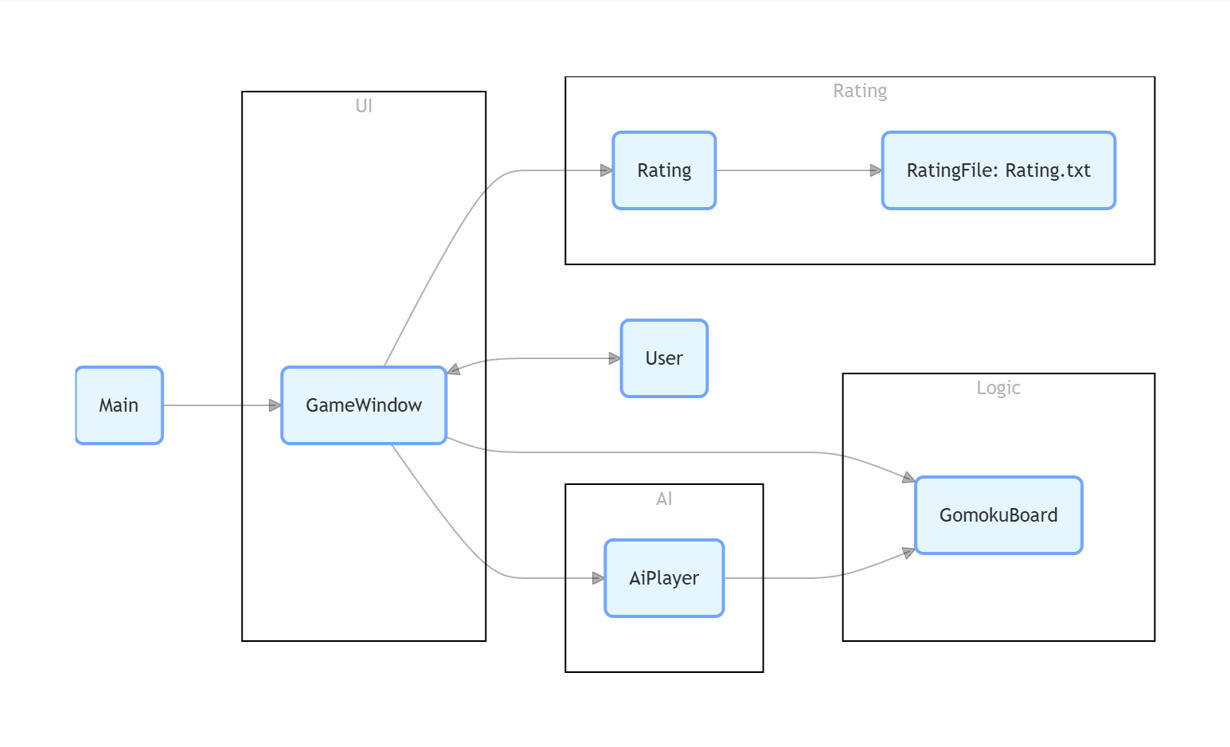
\includegraphics[width=0.9\textwidth]{structure.png}
    \caption{系统架构图}
\end{figure}

\subsection{核心类设计}
\begin{itemize}
    \item \textbf{GomokuBoard}:棋盘状态管理、落子逻辑、胜负判定
    \item \textbf{AiPlayer}:位置评估算法、最优落子点计算
    \item \textbf{GameWindow}:界面绘制、事件处理、游戏流程控制
    \item \textbf{Rating}:胜率计算、数据持久化
\end{itemize}
\subsection{AI评估算法}
采用基于规则的评估函数,考虑因素:
\begin{enumerate}
    \item \textbf{防守优先级}:优先阻断对手四连(100000分)
    \item \textbf{进攻机会}:构建自身连珠(优先构建五连999999分)
    \item \textbf{位置价值}:中心区域权重更高
\end{enumerate}

评分权重矩阵:
\[
\text{Score} = \sum_{\text{方向}} \begin{cases} 
100000 & \text{对手4连} \\
10000 & \text{对手活3} \\
5000 & \text{AI活3/4连} \\
500 & \text{AI活2}
\end{cases} + 10 \times (n - |x - c| - |y - c|)
\]

\subsection{胜率统计算法}
\[
\text{胜率} = \frac{Y}{Y + N} \times 100\%
\]
\begin{itemize}
    \item $Y$:从Rating.txt读取的"Y"行数
    \item $N$:从Rating.txt读取的"N"行数
\end{itemize}

\section{程序实现}
\subsection{开发环境}
\begin{itemize}
    \item 操作系统:Linux
    \item 编译器:g++
    \item GUI框架:Qt 5.15
    \item 构建工具:Makefile
\end{itemize}

\subsection{关键实现}
\subsubsection{棋盘绘制}
使用QPainter实现高质量棋盘渲染:
\begin{lstlisting}[language=C++]
void GameWindow::drawBoard(QPainter &painter) {

    painter.fillRect(..., QBrush(QColor(210, 180, 140, 180)));

    for (int i = 0; i < m_board.size(); ++i) {
        painter.drawLine(...);
        painter.drawLine(...);
    }

    painter.drawEllipse(QPoint(x, y), 4, 4);
}
\end{lstlisting}
\subsubsection{棋盘底层逻辑}
gomokuboard.h
\begin{lstlisting}[language=C++]
#ifndef GOMOKU_BOARD_H
#define GOMOKU_BOARD_H

#include <QVector>

class GomokuBoard {
public:
    enum Piece { Empty, Black, White };

    GomokuBoard(int size = 15);
    virtual ~GomokuBoard() = default;

    bool placePiece(int x, int y, Piece piece);
    bool checkWin(int x, int y) const;
    void reset();

    int size() const { return m_size; }
    Piece pieceAt(int x, int y) const { return m_board[x][y]; }

protected:
    QVector<QVector<Piece>> m_board;
    int m_size;
};

#endif
\end{lstlisting}
gomokuboard.cpp
\begin{lstlisting}[language=C++]
#include "gomokuboard.h"

GomokuBoard::GomokuBoard(int size) : m_size(size) {
	reset();
}

void GomokuBoard::reset() {
	m_board.resize(m_size);
	for (auto &row : m_board) {
		row.resize(m_size);
		row.fill(Empty);
	}
}

bool GomokuBoard::placePiece(int x, int y, Piece piece) {
	if (x < 0 || x >= m_size || y < 0 || y >= m_size || m_board[x][y] != Empty) {
		return false;
	}
	m_board[x][y] = piece;
	return true;
}

bool GomokuBoard::checkWin(int x, int y) const {
    Piece currentPiece = m_board[x][y];
    if (currentPiece == Empty) {
        return false;
    }
    const int directions[4][2] = {{1,0}, {0,1}, {1,1}, {1,-1}};
    
    for (auto &dir : directions) {
        int Count = 1;
        int dx = dir[0], dy = dir[1];

        for (int i = 1; i < 5; ++i) {
            int nx = x + dx * i, ny = y + dy * i;
            if (nx < 0 || nx >= size() || ny < 0 || ny >= size()) break;
            if (pieceAt(nx, ny) == currentPiece) {
                Count++;
            } else {
                break;
            }
        }

        for (int i = 1; i < 5; ++i) {
            int nx = x - dx * i, ny = y - dy * i;
            if (nx < 0 || nx >= size() || ny < 0 || ny >= size()) break;
            if (pieceAt(nx, ny) == currentPiece) {
                Count++;
            } else {
                break;
            }
        }
        if(Count >= 5) return true;
    }
    return false;
}
\end{lstlisting}
\subsubsection{AI决策流程}
\begin{enumerate}
    \item 遍历所有空位
    \item 计算每个位置的攻防评分
    \item 选择最高分位置
    \item 随机选择最优位置(防预测)
\end{enumerate}
\begin{lstlisting}[language=C++]
QPoint AiPlayer::calculateAIMove(GomokuBoard m_board) {
	int bestScore = -1;
	QVector<QPoint> bestMoves;
	
	for (int x = 0; x < m_board.size(); ++x) {
		for (int y = 0; y < m_board.size(); ++y) {
			if (m_board.pieceAt(x, y) == GomokuBoard::Empty) {
				int score = evaluatePosition(x, y, GomokuBoard::White,m_board);
				if (score > bestScore) {
					bestScore = score;
					bestMoves.clear();
					bestMoves.append(QPoint(x, y));
				} else if (score == bestScore) {
					bestMoves.append(QPoint(x, y));
				}
			}
		}
	}

	if (!bestMoves.isEmpty()) {
		int randomIndex = QRandomGenerator::global()->bounded(bestMoves.size());
		return bestMoves[randomIndex];
	}
	return QPoint(-1, -1);
}
int AiPlayer::evaluatePosition(int x, int y, GomokuBoard::Piece aiPiece,GomokuBoard m_board) {
	GomokuBoard::Piece humanPiece = (aiPiece == GomokuBoard::White) ? GomokuBoard::Black : GomokuBoard::White;
	int score = 0;
	
	const int directions[4][2] = {{1,0}, {0,1}, {1,1}, {1,-1}};
	
	for (auto &dir : directions) {
		int dx = dir[0], dy = dir[1];
		int aiCount = 1, humanCount = 1;
		bool aiBlocked = false, humanBlocked = false;

		for (int i = 1; i < 5; ++i) {
			int nx = x + dx * i, ny = y + dy * i;
			if (nx < 0 || nx >= m_board.size() || ny < 0 || ny >= m_board.size()) break;
			if (m_board.pieceAt(nx, ny) == aiPiece) {
				aiCount++;
			} else {
				if (m_board.pieceAt(nx, ny) == humanPiece) aiBlocked = true;
				break;
			}
		}

		for (int i = 1; i < 5; ++i) {
			int nx = x - dx * i, ny = y - dy * i;
			if (nx < 0 || nx >= m_board.size() || ny < 0 || ny >= m_board.size()) break;
			if (m_board.pieceAt(nx, ny) == aiPiece) {
				aiCount++;
			} else {
				if (m_board.pieceAt(nx, ny) == humanPiece) aiBlocked = true;
				break;
			}
		}
		
		for (int i = 1; i < 5; ++i) {
			int nx = x + dx * i, ny = y + dy * i;
			if (nx < 0 || nx >= m_board.size() || ny < 0 || ny >= m_board.size()) break;
			if (m_board.pieceAt(nx, ny) == humanPiece) {
				humanCount++;
			} else {
				if (m_board.pieceAt(nx, ny) == aiPiece) humanBlocked = true;
				break;
			}
		}

		for (int i = 1; i < 5; ++i) {
			int nx = x - dx * i, ny = y - dy * i;
			if (nx < 0 || nx >= m_board.size() || ny < 0 || ny >= m_board.size()) break;
			if (m_board.pieceAt(nx, ny) == humanPiece) {
				humanCount++;
			} else {
				if (m_board.pieceAt(nx, ny) == aiPiece) humanBlocked = true;
				break;
			}
		}
		

		if (humanCount >= 4) score += 100000;
		else if (humanCount == 3 && !humanBlocked) score += 10000;
		else if (humanCount == 2 && !humanBlocked) score += 1000;

		if(aiCount == 5) score += 999999;
		else if (aiCount >= 4) score += 5000;
		else if (aiCount == 3 && !aiBlocked) score += 5000;
		else if (aiCount == 2 && !aiBlocked) score += 500;
	}
	
	int center = m_board.size() / 2;
	int distanceToCenter = std::abs(x - center) + std::abs(y - center);
	score += (m_board.size() - distanceToCenter) * 10;
	
	return score;
}
\end{lstlisting}
\subsubsection{胜率计算}
\begin{lstlisting}[language=C++]
Rating::Rating(): rating(0), Y(0), N(0){
	std::string filename = "Rating.txt";
	std::ifstream file(filename);
	if (!file) {
		std::ofstream createFile(filename);
		if (createFile) {
			createFile.close();
			file.open(filename);
		}
	}
	std::string line;
	while (std::getline(file, line)) {
		if(line[0] == 'Y')Y++;
		if(line[0] == 'N')N++;
	}
	file.close();
	if (N == 0 && Y == 0) {
		rating = 0;
		message = QString("无信息");
		return;
	} else if (Y == 0) {
		rating = 0;
	} else if (N == 0) {
		rating = 100;
	} else {
		rating = Y / (Y + N) * 100;
	}
	message = QString("您的人机对战胜率为 %1 %").arg(rating, 0, 'f', 2);
}

void Rating::ShowRating(){
	QMessageBox msgBox;
	msgBox.setWindowTitle("胜率");
	msgBox.setText(QString("%1\nYes确认,No清空胜率").arg(message));
	msgBox.setStandardButtons(QMessageBox::Yes | QMessageBox::No);
	msgBox.setDefaultButton(QMessageBox::Yes);
	int ret = msgBox.exec();
	if (ret == QMessageBox::No) {
		std::ofstream file("Rating.txt", std::ios::trunc);
		if (!file) {
			return;
		}
		file.close();
	}
}
\end{lstlisting}

\section{程序测试}
\subsection{测试用例}
\begin{table}[h]
    \centering
    \begin{tabular}{lll}
        \toprule
        \textbf{测试项} & \textbf{预期结果} & \textbf{实际结果} \\
        \midrule
        人机对战-玩家胜利 & 胜率记录增加 & 符合 \\
        五连珠检测 & 正确识别所有方向 & 通过 \\
        边界落子 & 无崩溃 & 通过 \\
        \bottomrule
    \end{tabular}
    \caption{测试结果}
\end{table}

\subsection{界面测试}
\begin{figure}[htbp]
    \centering
    \begin{subfigure}[b]{0.3\textwidth}
        \centering
        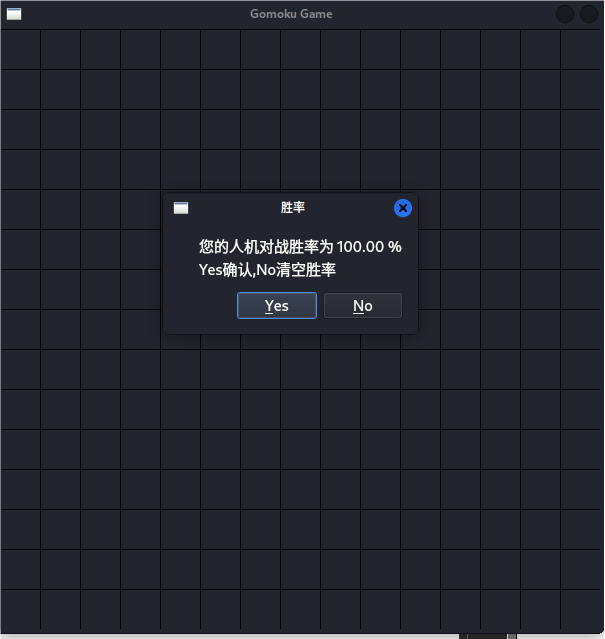
\includegraphics[width=\textwidth]{screenshoot1.png}
        \caption{图1}
        \label{fig:image1}
    \end{subfigure}%
    \hfill
    \begin{subfigure}[b]{0.3\textwidth}
        \centering
        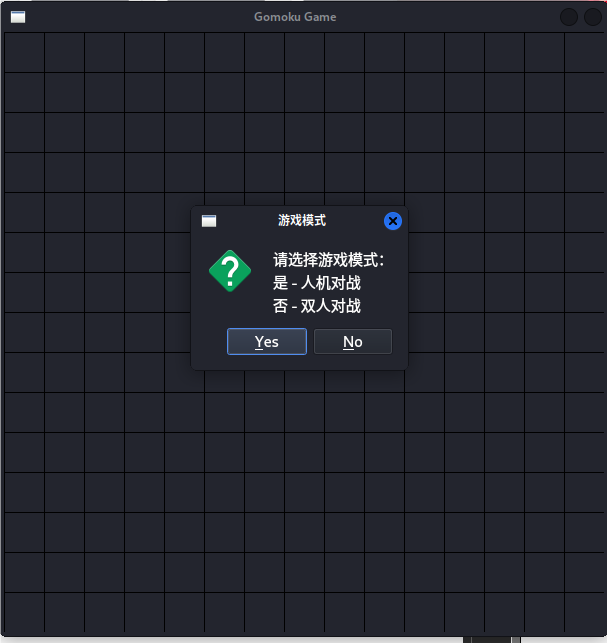
\includegraphics[width=\textwidth]{screenshoot2.png}
        \caption{图2}
        \label{fig:image2}
    \end{subfigure}%
    \hfill
    \begin{subfigure}[b]{0.3\textwidth}
        \centering
        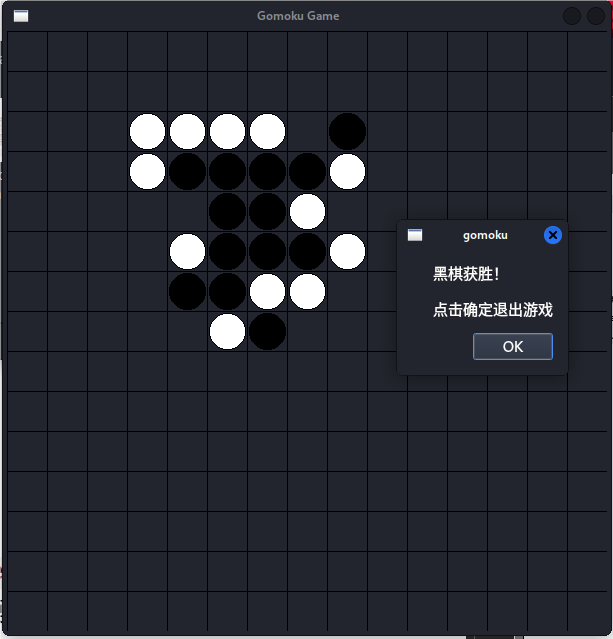
\includegraphics[width=\textwidth]{screenshoot3.png}
        \caption{图3}
        \label{fig:image3}
    \end{subfigure}
    \caption{测试图例}
    \label{fig:allimages}
\end{figure}

\section{任务分工}
\begin{itemize}
    \item \textbf{2410120028 侯成霖}:负责底层逻辑,算法,界面开发(GomokuBoard, AiPlayer,GameWindow),Latex文档 贡献度60\%
    \item \textbf{2410120036 陶永豪}:负责文件处理,界面开发(GameWindow,Rating),PPT 贡献度40\%
\end{itemize}

\section{经验总结}
\subsection{遇到的问题与解决}
\begin{itemize}
    \item \textbf{AI只下左上角}:调整分值评估,越在中间的评分越高
    \item \textbf{边界检测错误}:增加边界检查条件
    \item \textbf{显示程序内存溢出}:调整大小加入检查
\end{itemize}

\subsection{改进方向}
\begin{itemize}
    \item 增加难度级别选择
    \item 实现悔棋功能
    \item 添加音效和动画
    \item 优化AI算法(Minimax+Alpha-Beta剪枝)
\end{itemize}

\subsection{总结体会}
通过本项目,我们深入掌握了:
\begin{itemize}
    \item Qt框架的图形编程技术
    \item 游戏AI设计原则
    \item 面向对象设计模式
    \item 团队协作开发流程
\end{itemize}
五子棋虽规则简单,但在实现过程中涉及到算法优化、用户体验、代码架构等多方面挑战,是一次宝贵的开发经验。

\end{document}